\subsection{Undicesimo sprint}

\begin{minipage}{\textwidth}
  Di seguito è riportata la distribuzione delle ore per ciascun membro del team, accumulate in totali per persona e per ruolo:
  \begin{table}[H]
    \begin{tabularx}{\textwidth}{|c|*{6}{>{\centering}X|}c|}
      \hline
      \multicolumn{8}{|c|}{\textbf{Consuntivo orario}} \\
      \hline
      \textbf{Membro del team} & \textbf{Re} & \textbf{Am} & \textbf{An} & \textbf{Pt} & \textbf{Pr} & \textbf{Ve} & \textbf{Totale per persona} \\
      \hline
      Riccardo Cavalli & 0 & 0 & 1 & 2 & 2 & 2 & 7 \\
      \hline
      Raul Pianon & 0 & 0 & 0 & 7 & 2 & 1 & 10 \\
      \hline
      Martina Dall'Amico & 0 & 0 & 0 & 6 & 3 & 1 & 10 \\
      \hline
      Marco Cristo & 0 & 2 & 0 & 4 & 4 & 0 & 10 \\
      \hline
      Sebastiano Lewental & 0 & 1 & 0 & 2 & 4 & 3 & 10 \\
      \hline
      Mattia Zecchinato & 3 & 0 & 0 & 3 & 1 & 3 & 10 \\
      \hline
      Tommaso Stocco & 2 & 0 & 0 & 6 & 2 & 0 & 10 \\
      \hline
      \textbf{Totale ore per ruolo} & 5 & 3 & 1 & 30 & 18 & 10 & \textbf{67} \\
      \hline
    \end{tabularx}
    \caption{Sprint 11 - Consuntivo orario}
  \end{table}
  \end{minipage}

  \begin{figure}[H]
    \centering
    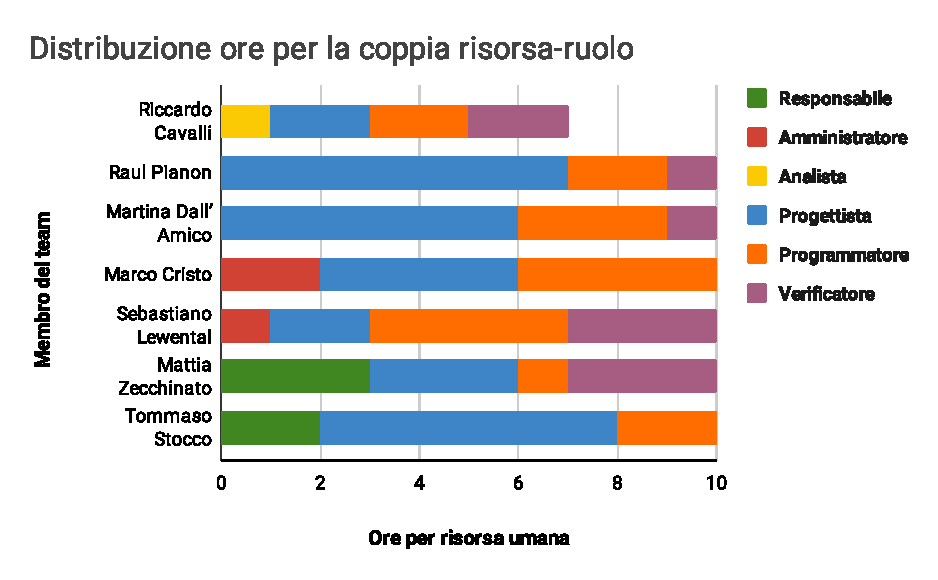
\includegraphics[width=0.90\textwidth]{assets/Consuntivo/Sprint-11/distribuzione_ore_risorsa_ruolo.pdf}
    \caption{Sprint 11 - Istogramma della distribuzione oraria per la coppia risorsa-ruolo}
  \end{figure}

  \begin{figure}[H]
    \centering
    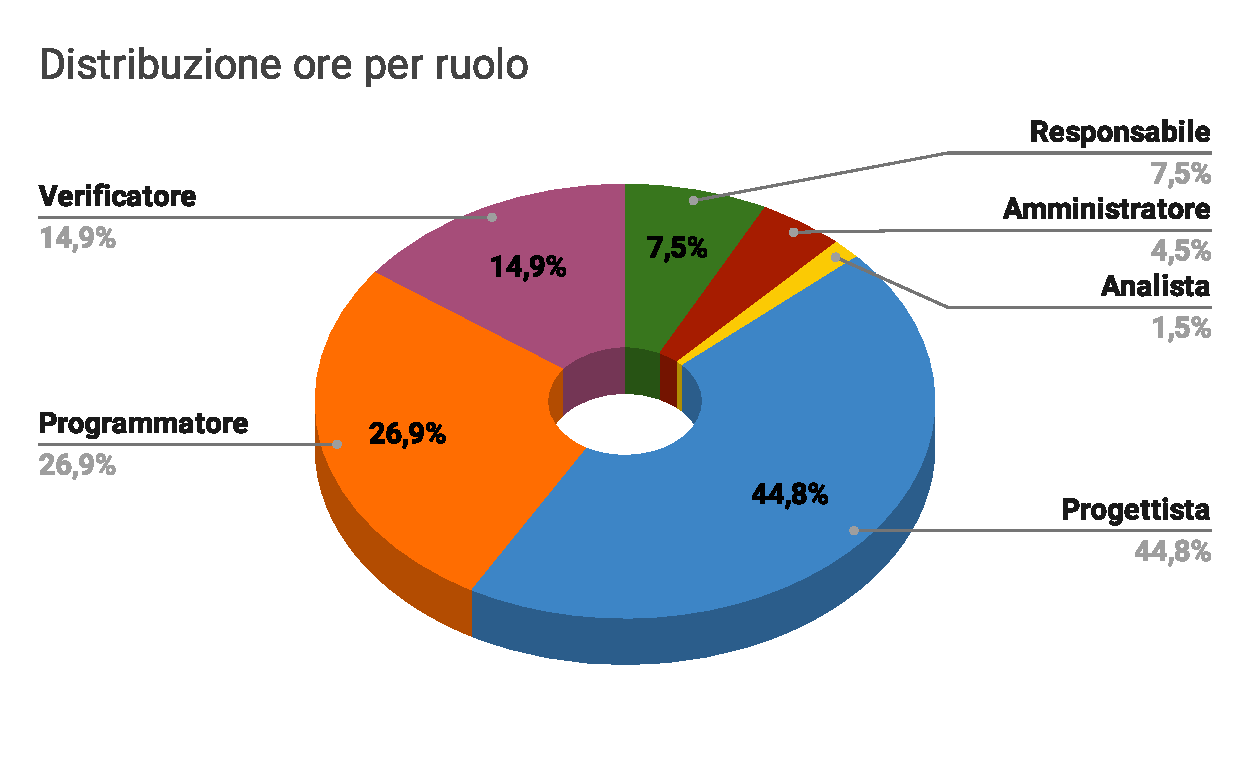
\includegraphics[width=0.90\textwidth]{assets/Consuntivo/Sprint-11/distribuzione_ore_ruolo.pdf}
    \caption{Sprint 11 - Areogramma della distribuzione oraria per ruolo}
  \end{figure}

  \begin{minipage}{\textwidth}
  Di seguito è riportato il consuntivo economico dell'undicesimo \glossario{sprint}:
  \begin{table}[H]
  \begin{adjustwidth}{-0.5cm}{-0.5cm}
    \centering
    \begin{tabular}{|P{2.9cm}|P{2.3cm}|P{2.5cm}|P{2.3cm}|>{\arraybackslash}P{2.5cm}|}
      \hline
      \multicolumn{5}{|c|}{\textbf{Consuntivo economico}} \\
      \hline
      \textbf{Ruolo} & \textbf{Ore per ruolo} & \textbf{Delta ore preventivo - consuntivo} & \textbf{Costo (in \texteuro)} & \textbf{Delta costo preventivo - consuntivo (in \texteuro)} \\
      \hline
      \Responsabile[U]{} & 5 & -1 & 150,00 & -30,00 \\ \hline
      \Amministratore[U]{} & 3 & 1 & 60,00 & 20,00 \\ \hline
      \Analista[U]{} & 1 & 1 & 25,00 & 25,00 \\ \hline
      \Progettista[U]{} & 30 & 0 & 750,00 & 0,00 \\ \hline
      \Programmatore[U]{} & 18 & -1 & 270,00 & -15,00 \\ \hline
      \Verificatore[U]{} & 10 & 0 & 150,00 & 0,00 \\ \hline
      \textbf{Totale} & \textbf{67} & 0 & \textbf{1.405,00} & 0,00 \\ \hline
      \textbf{Restante} & 152 & / & 3.015,00 & / \\ \hline
      \textbf{Sprint pregressi} & 427 & / & 8.600,00 & / \\ \hline
    \end{tabular}
    \caption{Sprint 11 - Consuntivo economico}
  \end{adjustwidth}
  \end{table}
  \end{minipage}

  \begin{figure}[H]
    \centering
    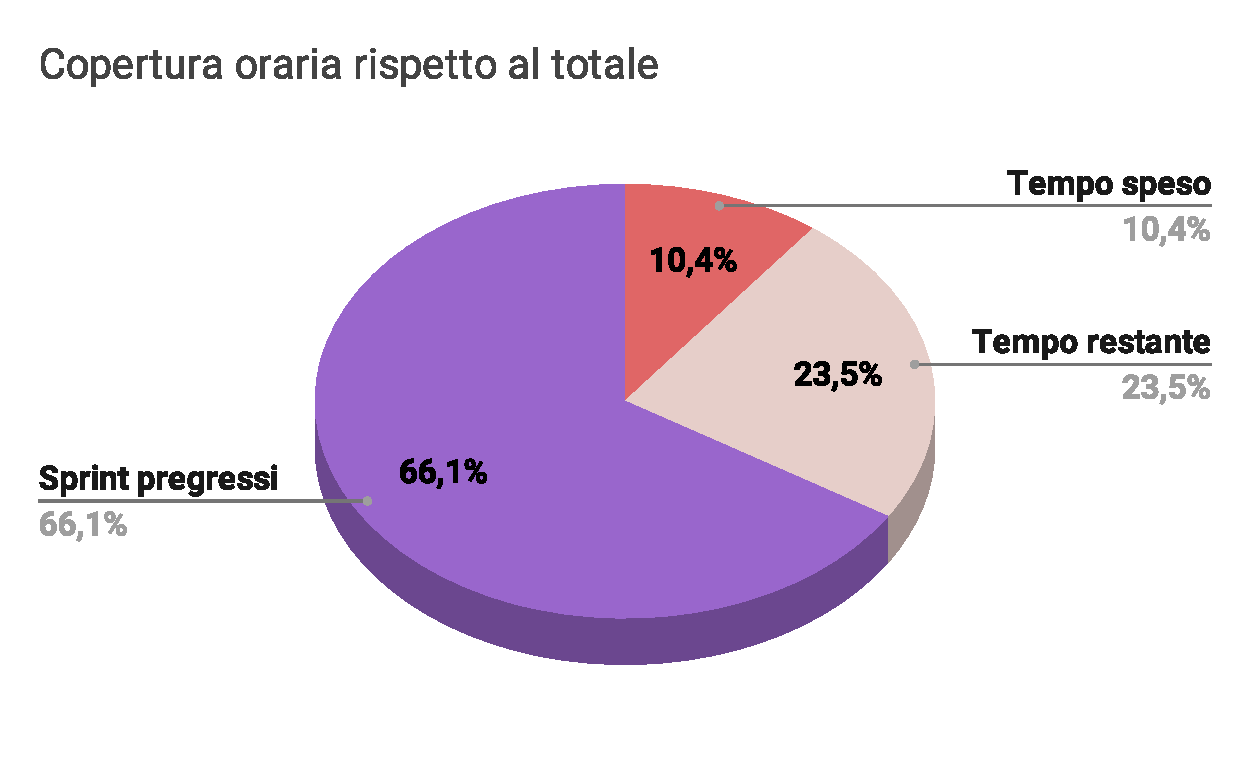
\includegraphics[width=0.90\textwidth]{assets/Consuntivo/Sprint-11/copertura_oraria.pdf}
    \caption{Sprint 11 - Areogramma del tempo speso (in ore) rispetto al totale}
  \end{figure}

  \begin{figure}[H]
    \centering
    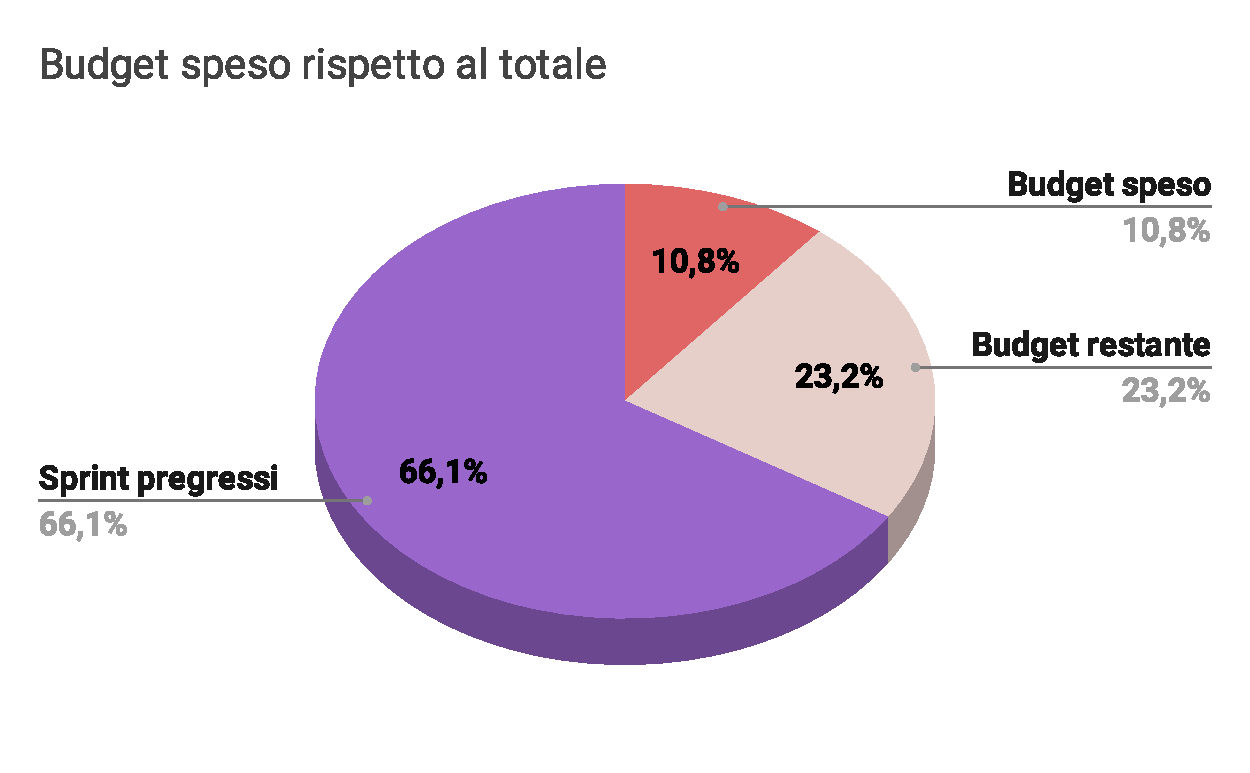
\includegraphics[width=0.90\textwidth]{assets/Consuntivo/Sprint-11/budget_speso.pdf}
    \caption{Sprint 11 - Areogramma del budget speso rispetto al totale}
  \end{figure}

  \begin{minipage}{\textwidth}
    Di seguito sono riportate le ore rimanenti per la coppia risorsa-ruolo:
    \begin{table}[H]
      \begin{tabularx}{\textwidth}{|c|*{6}{>{\centering}X|}c|}
        \hline
        \multicolumn{8}{|c|}{\textbf{Ore rimanenti per la coppia risorsa-ruolo}} \\
        \hline
        \textbf{Membro del team} & \textbf{Re} & \textbf{Am} & \textbf{An} & \textbf{Pt} & \textbf{Pr} & \textbf{Ve} & \textbf{Totale per persona} \\
        \hline
        Riccardo Cavalli & 0 & 1 & 2 & 5 & 7 & 4 & 19 \\
        \hline
        Raul Pianon & 2 & 1 & 1 & 6 & 7 & 3 & 20 \\
        \hline
        Martina Dall'Amico & 2 & 1 & 1 & 6 & 7 & 6 & 23 \\
        \hline
        Marco Cristo & 1 & 2 & 0 & 7 & 6 & 5 & 21 \\
        \hline
        Sebastiano Lewental & 2 & 2 & 1 & 5 & 7 & 5 & 22 \\
        \hline
        Mattia Zecchinato & 2 & 2 & 2 & 6 & 5 & 5 & 22 \\
        \hline
        Tommaso Stocco & 1 & 0 & 3 & 9 & 7 & 5 & 25 \\
        \hline
        \textbf{Totale ore per ruolo} & 10 & 9 & 10 & 44 & 46 & 33 & \textbf{152} \\
        \hline
      \end{tabularx}
      \caption{Sprint 11 - Ore rimanenti per la coppia risorsa-ruolo}
    \end{table}
  \end{minipage}

\subsubsection{Revisione delle attività}

Nell'arco dell'undicesimo \glossario{sprint}, il team ha svolto le seguenti attività:
\begin{itemize}
  \item Selezione del modello architetturale per il \glossario{back-end};
  \item Stesura sezione architettura nel documento di \ST;
  \item Completata progettazione logica del back-end;
  \item Completata progettazione di dettaglio del \glossario{front-end};
  \item Avanzamento codifica front-end e back-end;
  \item Gestione centralizzata degli errori a front-end;
  \item Definizione di interfacce e tipi con \glossario{TypeScript};
  \item Consuntivo \glossario{sprint} 10;
  \item Stesura verbali interni;
  \item Aggiornamento dei grafici nel \PdQ;
  \item Configurazione dell'ambiente di test front-end (Cypress) e back-end (pytest);
  \item Progettazione dei test di unità;
  \item Configurazione di strumenti per automatizzare la formattazione e il \glossario{linting} del codice;
  \item Definizione di un workflow su \glossario{GitHub} per automatizzare formattazione, linting e test;
  \item Organizzazione di un incontro in presenza a Padova;
  \item Stesura del \MU\ nelle seguenti sezioni:
  \begin{itemize}
    \item Chat;
    \item Gestione \glossario{dizionari dati};
    \item Configurazione delle impostazioni;
    \item Visualizzazione mobile.	
  \end{itemize}	
  \item Configurazione di SonarCloud per calcolare alcune metriche di qualità del codice (complessità ciclomatica, duplicazione, sicurezza);
  \item Implementazione del modello architetturale scelto;
  \item Implementazione dei \glossario{design pattern} ritenuti pertinenti;
  \item Stesura del diagramma delle classi;
  \item Testing dei componenti front-end e back-end;
  \item Stesura tracciamento dei requisiti nel documento di \ST;
  \item Completata sezione \glossario{debug} (front-end);
  \item Separazione delle responsabilità del metodo di generazione del \glossario{prompt}.
\end{itemize}

\subsubsection{Retrospettiva}

\par Di seguito sono riportati i risultati del questionario di valutazione dello \glossario{sprint}:
\begin{itemize}
  \item Organizzazione dello sprint - Valutazione: 9;
  \item Conduzione dei meeting interni - Valutazione: 9;
  \item Impegno e partecipazione dei singoli membri - Valutazione: 8;
  \item Tutti i membri del team erano a conoscenza delle proprie mansioni;
  \item La numerosità delle riunioni è risultata adeguata per tutti i membri del gruppo;
  \item Le riunioni sono state organizzate quasi sempre con il giusto preavviso;
  \item Rispetto allo sprint precedente, la discrepanza tra le ore spese e quelle effettivamente produttive è aumentata.
\end{itemize}

\vspace{0.5\baselineskip}
\par A seguire le \textbf{analisi a posteriori} dell'undicesimo \glossario{sprint}:
\begin{itemize}
  \item La configurazione e la progettazione dei test del front-end hanno richiesto più risorse del previsto, portando a un impiego di ore superiore rispetto a quelle effettivamente produttive. Nonostante ciò, il gruppo è riuscito a completare i task più urgenti entro i tempi stabiliti;
  \item La suddivisione del team in sottogruppi di tre persone si è dimostrata una scelta proficua. Durante lo sprint, il team ha implementato con successo il modello architetturale e i design pattern selezionati, completando anche il diagramma delle classi;
  \item L'adozione di analisi statica e dinamica ha rafforzato la capacità del gruppo di individuare potenziali difetti nel software;
  \item L'integrazione continua nell'ambiente condiviso e l'uso delle \glossario{pull request} come spazio di discussione hanno favorito la collaborazione e il miglioramento continuo;
  \item Il team ha integrato SonarCloud con \glossario{GitHub}, introducendo un ulteriore livello di verifica nelle pull request. In questo modo, i test sviluppati dal gruppo (potenzialmente non esaustivi) sono supportati da controlli effettuati da strumenti di terze parti;
  \item Avviando la fase di codifica, il gruppo ha confermato la validità delle decisioni prese durante la \glossario{RTB}. In particolare, l'adozione di \glossario{TypeScript} anziché JavaScript ha contribuito a ridurre il numero di errori imprevisti e a migliorare la robustezza del codice;
  \item Durante l'incontro in presenza, il team ha condiviso idee e valutazioni approfondite, che si sono rivelate essenziali per un'implementazione efficiente dell'architettura.
\end{itemize}

\subsubsection{Aggiornamento pianificazione e preventivo}
\par Il team ha definito un piano d'azione per migliorare l'organizzazione e la produttività del prossimo \glossario{sprint}:
\begin{itemize}
  \item Preservare la suddivisione in sottogruppi, ciascuno incaricato di testare le funzionalità del front-end e del back-end;
  \item Migliorare i commenti del codice per facilitare la manutenibilità e la leggibilità.
\end{itemize}

\paragraph*{Pianificazione futura:}
\par Il team ha completato l'implementazione del modello architetturale in un tempo inferiore rispetto alle previsioni. Di conseguenza, nel prossimo \glossario{sprint}, il gruppo concentrerà i propri sforzi sulle attività di testing. Inoltre, il documento di \ST\ sarà ampliato per approfondire  le scelte progettuali adottate.

\paragraph*{Preventivo "a finire" (\sezione{sec:stima_temporale}):}
\par Il gruppo ha ritenuto non necessaria una ridistribuzione delle ore, poiché i ruoli di progettista, programmatore e verificatore sono stati assegnati in base alla pianificazione futura. Per quanto riguarda il budget, l'Estimate at Completion (EAC) è rimasto al di sotto della soglia prevista di 13.020,00 €.

\paragraph*{Gestione dei rischi (\sezione{sec:analisi_rischi}):}
\par Durante l'undicesimo \glossario{sprint}, i seguenti rischi sono stati gestiti con successo:
\begin{itemize}
  \item \textbf{RO3: Sottostima delle risorse necessarie per un'attività}: il gruppo ha sottostimato le risorse necessarie per la configurazione dell'ambiente di test del front-end, con il rischio di compromettere l'esecuzione dei task successivi. Per affrontare questo problema, il team ha suddiviso l'attività in sotto-task e ha organizzato una serie di riunioni dedicate. Queste azioni hanno permesso di completare l'incarico con il minor ritardo possibile;
  \item \textbf{RT3 - Malfunzionamenti software}: la configurazione e l'esecuzione dei test hanno provocato malfunzionamenti software, in particolare conflitti tra le dipendenze installate. Nonostante l'inesperienza del gruppo, gli errori sono stati risolti tempestivamente seguendo le procedure indicate nelle \NdP.
\end{itemize}